\chapter{File Handling: Making Programs Remember}

\section{Introduction: Real-Life Hook}

Rafi writes his homework on paper.
Even if he sleeps, wakes up, or goes to school the next day,  
his writing is still there.

But when Rafi writes a Python program:
\begin{itemize}
    \item The program forgets everything after closing
    \item All data disappears
\end{itemize}

How can a program remember things like humans remember notes?

The answer is \textbf{File Handling}.

\section{What Is File Handling?}

\begin{definition}{File Handling}
File handling is the process of \textbf{creating, reading, writing, and storing data in files}.
\end{definition}

Using file handling, programs can:
\begin{itemize}
    \item Save data permanently
    \item Read stored information later
    \item Share data between programs
\end{itemize}

\section{Why File Handling Is Important}

Without file handling:
\begin{itemize}
    \item Programs forget everything
    \item Data is lost after execution
\end{itemize}

With file handling:
\begin{itemize}
    \item Data is stored safely
    \item Programs become useful in real life
\end{itemize}

Examples:
\begin{itemize}
    \item Saving exam results
    \item Storing login information
    \item Keeping attendance records
\end{itemize}

\section{What Is a File?}

A file is a place where data is stored permanently.

Examples:
\begin{itemize}
    \item \texttt{notes.txt}
    \item \texttt{marks.csv}
    \item \texttt{data.txt}
\end{itemize}

\section{Opening a File in Python}

Python uses the \texttt{open()} function.

\begin{verbatim}
file = open("data.txt", "r")
\end{verbatim}

\textbf{Syntax:}
\begin{verbatim}
open(filename, mode)
\end{verbatim}

\section{File Modes}

\begin{center}
\begin{tabular}{|c|c|}
\hline
\textbf{Mode} & \textbf{Meaning} \\
\hline
r & Read \\
w & Write (overwrite) \\
a & Append \\
r+ & Read and write \\
\hline
\end{tabular}
\end{center}

\section{Writing to a File}

\begin{verbatim}
file = open("note.txt", "w")
file.write("Hello, this is my first file")
file.close()
\end{verbatim}

\begin{itemize}
    \item \texttt{write()} saves data
    \item \texttt{close()} closes the file
\end{itemize}

\section{Reading from a File}

\begin{verbatim}
file = open("note.txt", "r")
content = file.read()
print(content)
file.close()
\end{verbatim}

\section{Appending Data to a File}

\begin{verbatim}
file = open("note.txt", "a")
file.write("\nNew line added")
file.close()
\end{verbatim}

Append mode keeps old data and adds new data.

\section{Using \texttt{with} Statement (Best Practice)}

\begin{verbatim}
with open("note.txt", "r") as file:
    print(file.read())
\end{verbatim}

Advantages:
\begin{itemize}
    \item Automatically closes file
    \item Reduces errors
\end{itemize}

\section{Real-Life Example: Student Diary}

\begin{verbatim}
with open("diary.txt", "a") as file:
    file.write("Today I learned file handling\n")
\end{verbatim}

The program remembers daily learning.

\section{Mini-Project: Student Marks Record}

\textbf{Goal:} Save and read student marks.

\begin{verbatim}
with open("marks.txt", "w") as file:
    file.write("Rahim: 85\n")
    file.write("Karim: 90\n")

with open("marks.txt", "r") as file:
    print(file.read())
\end{verbatim}

Students learn:
\begin{itemize}
    \item Permanent data storage
    \item Read and write operations
\end{itemize}

\section{Common File Errors}

\begin{itemize}
    \item File not found
    \item Wrong file mode
    \item Forgetting to close file
\end{itemize}

\section{Diagram: File Handling Process}

\begin{center}
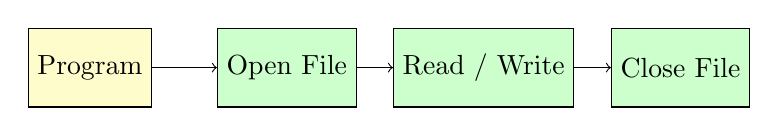
\begin{tikzpicture}[node distance=2.5cm]
\node (prog) [draw, rectangle, fill=yellow!20, minimum height=1cm] {Program};
\node (open) [draw, rectangle, fill=green!20, right of=prog, minimum height=1cm] {Open File};
\node (rw) [draw, rectangle, fill=green!20, right of=open, minimum height=1cm] {Read / Write};
\node (close) [draw, rectangle, fill=green!20, right of=rw, minimum height=1cm] {Close File};

\draw[->] (prog) -- (open);
\draw[->] (open) -- (rw);
\draw[->] (rw) -- (close);
\end{tikzpicture}
\end{center}

\section{Key Concepts}

\begin{itemize}
    \item File handling stores data permanently
    \item Files must be opened before use
    \item Always close files after use
    \item Use \texttt{with} for safety
\end{itemize}

\section{Common Beginner Mistakes}

\begin{itemize}
    \item Using wrong file mode
    \item Overwriting data accidentally
    \item Not handling missing files
\end{itemize}

\section{End-of-Chapter Exercises}

\subsection{Very Short Questions}

\begin{enumerate}
    \item What is file handling?
    \item Name any two file modes.
    \item Why is \texttt{close()} important?
\end{enumerate}

\subsection{Short Answer Questions}

\begin{enumerate}
    \item Explain file handling with a real-life example.
    \item Difference between write and append mode.
    \item What are the benefits of the \texttt{with} statement?
\end{enumerate}

\subsection{Activity-Based Exercises}

\begin{enumerate}
    \item Create a program to save your daily study notes.
    \item Store names of five friends in a file.
    \item Read a file and count number of lines.
\end{enumerate}

\section{Teacher Notes}

\marginnote{
\textbf{Learning Objectives}
\begin{itemize}
    \item Students understand file handling basics
    \item Students perform read and write operations
    \item Students use files for permanent storage
\end{itemize}

\textbf{Teaching Tips}
\begin{itemize}
    \item Compare with notebook memory
    \item Show file content physically
    \item Demonstrate data loss without files
\end{itemize}

\textbf{Assessment}
\begin{itemize}
    \item Correct file mode usage
    \item Proper file handling logic
\end{itemize}
}